\subsection{Feature-family importance}
For the final GBT-B model, Spark split importances were mapped from encoded
vector indices to feature families and normalized by total importance.
Current rainfall contributed 45.02\%, followed by threshold at 23.40\%,
rolling maxima at 10.27\% and rolling totals at 10.24\%
(Figure~\ref{fig:feature-family}). Station identity had no split importance
in this fitted model. Split importance measures feature use by the fitted
trees; it is not a causal measure. Correlated rainfall-history variables may
divide importance between them.

\begin{figure}[htbp]
\centering
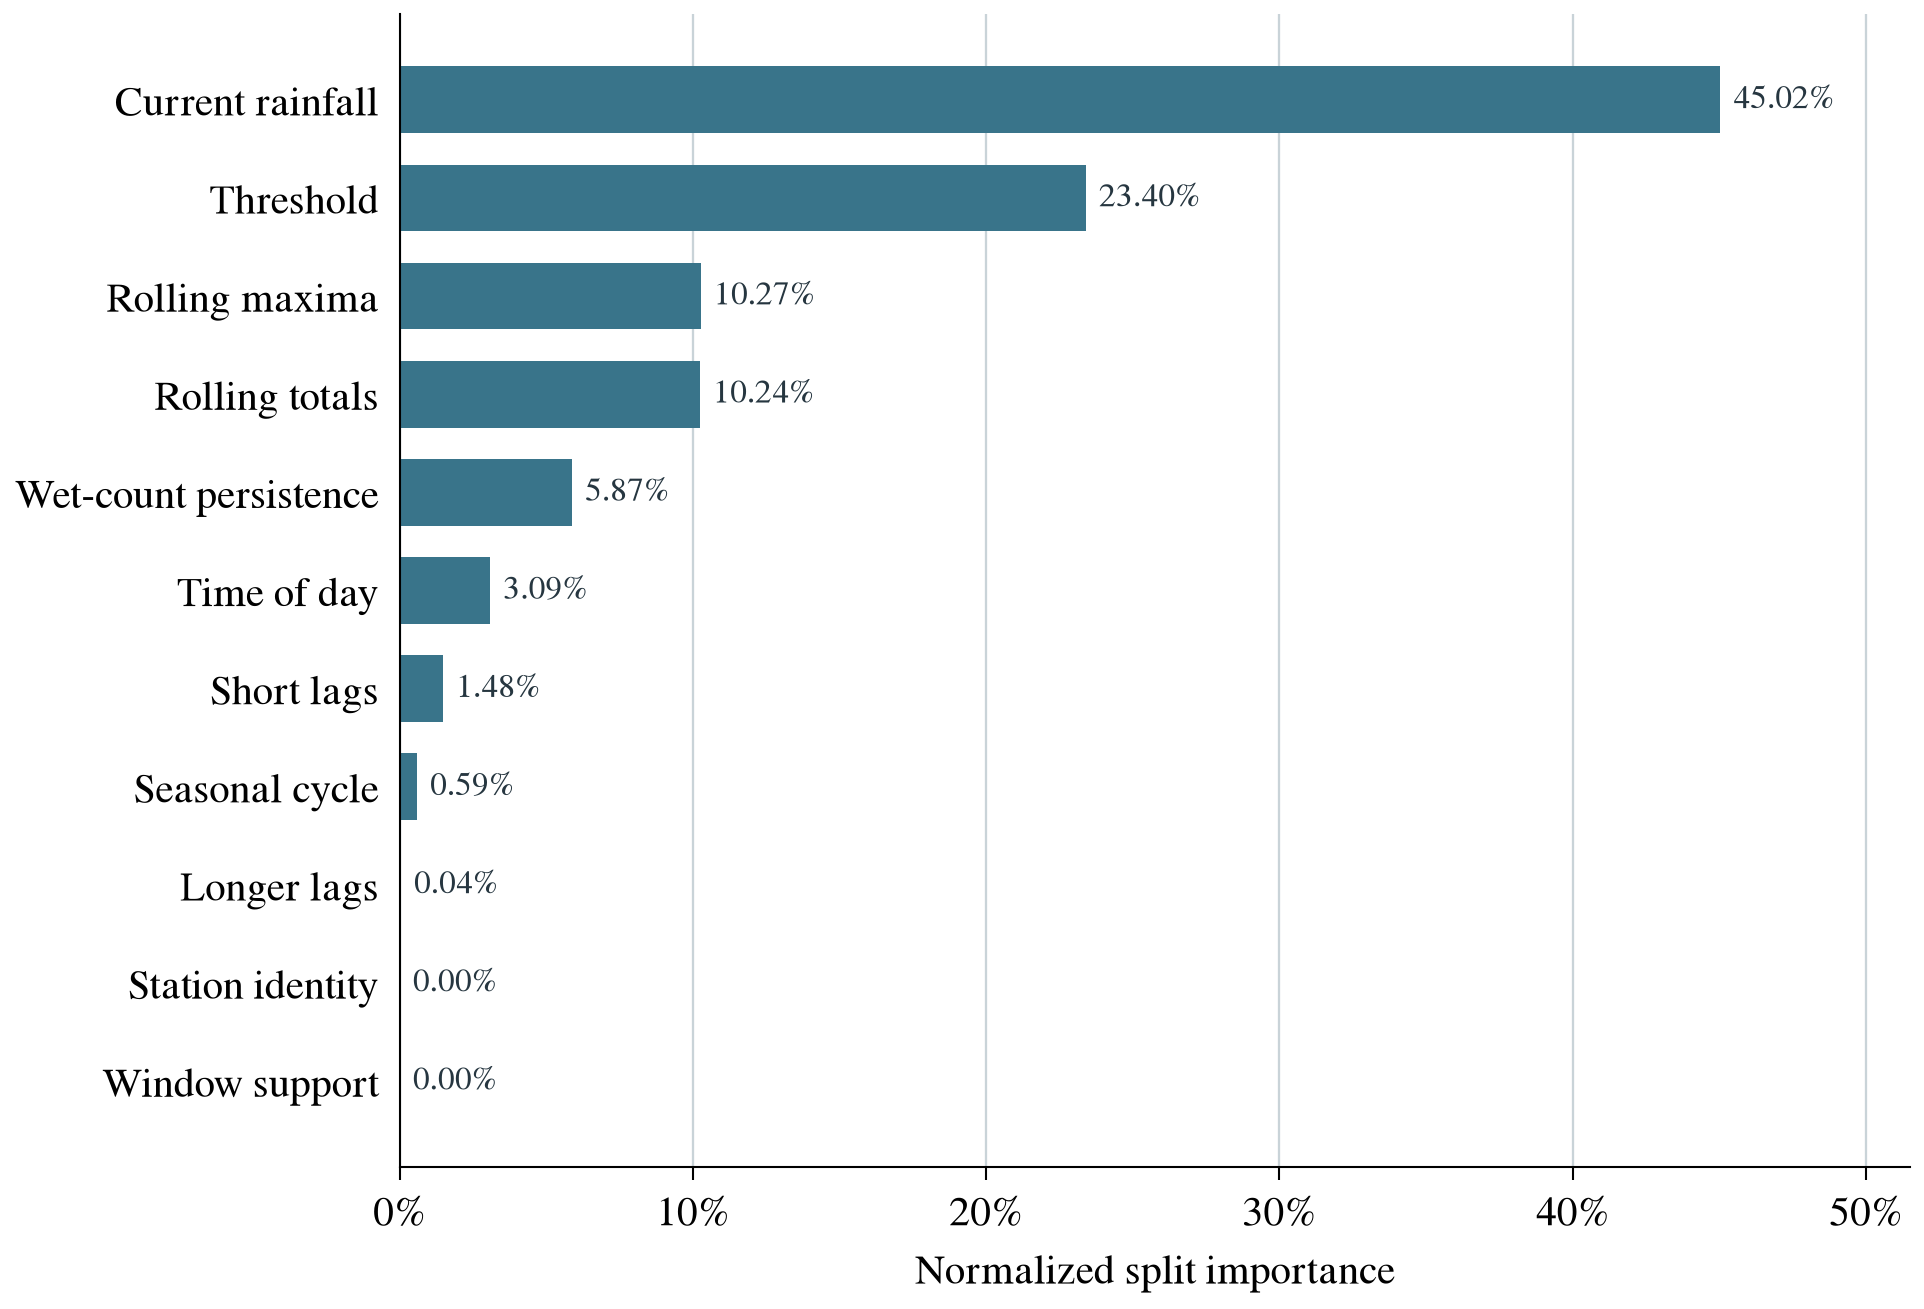
\includegraphics[width=0.88\linewidth]{figures/final/feature_family_importance.png}
\caption{Final GBT-B split importance aggregated by feature family after
mapping encoded feature-vector indices. Values are normalized shares of total
split importance.}
\label{fig:feature-family}
\end{figure}

